\section{Problem}
\markright{Problem}

This program demonstrates the use of constructors, copy constructors, and destructors in a C++ class. It defines a \texttt{Student} class with default and parameterized constructors, then creates multiple objects to show object initialization and copy behavior.

\subsubsection{Code}
\begin{lstlisting}[language=C++, numbers=left]
#include <iostream>

class Student {
    int id;

public:
    // Default Constructor
    Student() {
        id = 0;
        std::cout << "Default Constructor Called" << std::endl;
    }

    // Parameterized Constructor
    Student(int x) {
        id = x;
        std::cout << "Parameterized Constructor Called" << std::endl;
    }

    // Copy Constructor
    Student(const Student &obj) {
        id = obj.id + 1;
        std::cout << "Copy Constructor Called" << std::endl;
    }

    // Destructor
    ~Student() {
        std::cout << "Destructor Called for ID = " << id << std::endl;
    }
};


int main() {
    Student s1;        // Default Constructor

    Student s2(2408020); // Parameterized Constructor

    Student s3 = s2;   // Copy Constructor

    Student s4(s3); // Copy Constructor

    return 0;
}
\end{lstlisting}

\subsubsection{Output}
\begin{figure}[H]
    \centering
    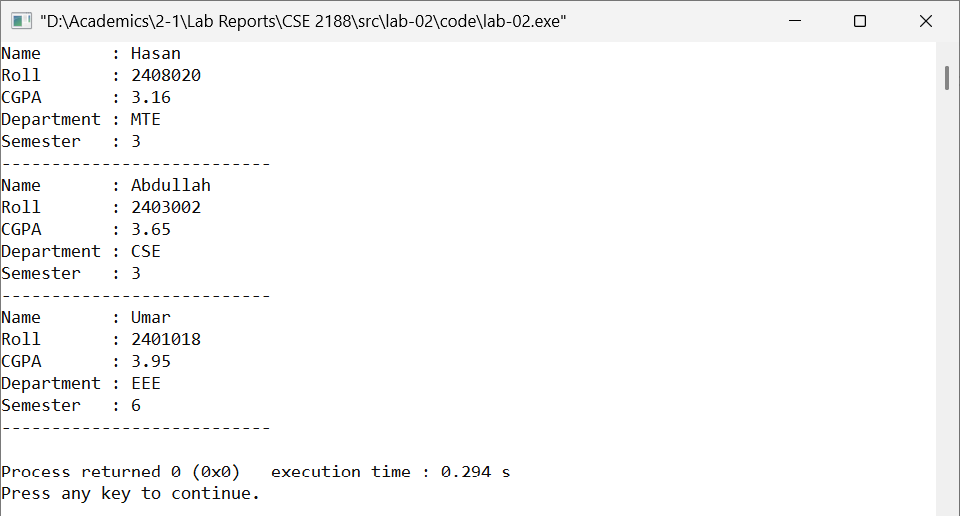
\includegraphics[width=0.8\textwidth]{lab-02/assets/output-student.png}
    \caption{Output showing default, parameterized, and copy constructor calls along with destructor execution.}
\end{figure}
